
\chapter{Fortbewegung}

\section{Fahrrad}

Fahrradfahren lohnt sich nicht nur, weil es die schnellste und
flexibelste Möglichkeit ist, in München voranzukommen, es ist auch
gesund, schont das Klima und macht Spaß.  Es ist auch deutlich
günstiger als die häufig überfüllten öffentlichen Nahverkehrsmittel:
Wenn man das Semester über Rad fährt spart man sich 141~€.

Damit kann man schon den ein oder anderen Drahtesel refinanzieren oder
hat zumindest eine Anzahlung für ein gutes, gebrauchtes Fahrrad. Dieses
findet man beispielsweise bei eBay, Polizei-, Bahnhofs- und
Wohnheimsversteigerungen oder auf einem der zahlreichen Flohmärkte in
München. 

München ist nicht nur Radlhauptstadt, sondern auch (gefühlte)
Kontrollierhauptstadt. Auf ausgeschilderten Strecken sollte man Schrittgeschwindigkeit
einhalten, sonst zahlt man schnell 15~€. Ohne Licht bei Nacht oder
Dunkelheit sowie auf der falschen Straßenseite fahren
(dies gilt auch auf der Leopold"~ / Ludwigstr.), kosten 20~€.  Vor allem nicht unterschätzen sollte man das Rotlicht
an Ampeln. Durch ignorieren des selben ist man schnell mal 100~€ los und sammelt
zusätzlich noch Punkte in Flensburg.

Ansonsten bleibt uns vor allem der Rat, euch nicht vom Münchner
Verkehrsverhalten anstecken zu lassen, sondern defensiv und rücksichtsvoll zu
fahren. Unsere zahlreichen Nahtoderlebnisse im Stadverkehr sind nicht
nachahmenswert.

\subsection*{Hier noch ein paar Tipps für den Münchner Straßenverkehr:}
\begin{itemize}
	\item Trambahnschienen werden bei Regen, Schnee und Glätte eine Todesfalle.
	\item Fußgänger schweben in eigenen Sphären. Die Autofahrer sind leider 
				manchmal ähnlich unvorhersehbar.
	\item Helme haben schon so Manchem das Leben gerettet.
	\item Um das Wiederfinden des Fahrrades zu erleichtern, sollte man es 
				abschließen.
\end{itemize}

Wenn du kein eigenes Fahrrad besitzt und dir auch keines kaufen möchtest, aber im
Stadtkern München wohnst, sind vielleicht die Leihräder der Deutschen Bahn,
namentlich Call a Bike \ref{callabike}, für dich interessant. Für 24,00~€ pro
Jahr bekommst du als Studikon den \emph{Pauschaltarif}, welcher dir erlaubt jedes
Fahrrad für die ersten 30~Minuten kostenfrei zu benutzen. Erst danach fällt der
reguläre Preis von 0,08~€ pro Minute an. In 30 Minuten kommt man in München mit dem Fahrrad
aber ganz schön weit.

Vorsicht gilt es aber bei der Rückgabe der Leihräder walten zu lassen: Ist das
Fahrrad mehr als 30 Meter von der nächsten Kreuzung abgestellt kostet das
5,00~€, außerhalb des Geschäftsgebietes 10,00~€ und außerhalb der Stadtgrenzen
auch schon Mal 25,00~€!

Neben Call a Bike von der Bahn gibt es auch Nextbike \ref{nextbike}, bei
welchen du das Fahrrad jedoch an festen Stationen wieder abstellen musst.

\begin{urlList}
	\urlItem{http://callabike-interaktiv.de}{callabike}
	\urlItem{http://nextbike.de}{nextbike}
\end{urlList}

%\begin{textblock*}{\paperwidth}(50mm,128mm)
%   \noindent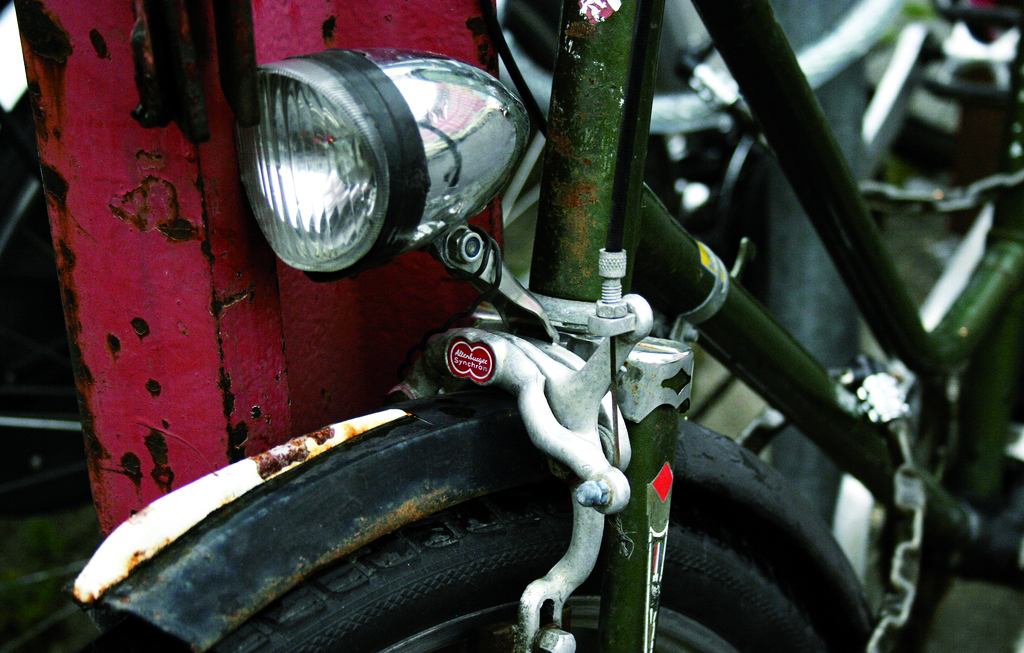
\includegraphics[width={\paperwidth-50mm}]{flickr/725703538_5b9a97ecf2_b}
%	\label{img_bike}
%\end{textblock*}


\section{MVV}
Der Münchner Verkehrsverbund ist der Träger des Großteils des ÖPNV in München.

\subsection*{Mit den öffentlichen Verkehrsmitteln in die Uni}\hfill\\
Die U-Bahnen U3 und U6 halten direkt am Hauptgebäude (Haltestelle Universität).
Die meisten anderen Gebäude sind ebenfalls mit U-Bahn, Bus oder Tram gut zu
erreichen. Genaueres zu den wichtigsten Gebäuden und naheliegenden Haltestellen
finden sich auf der am Ende dieses Heftes zu findenden Karte.

%Informationen zu den anfallenden Kosten für den MVV (Münchner Verkehrsverbund) findest du im Kapitel "`Semesterticket und Ausbildungstarif"'.
%\subsection*{Kosten}\hfill\\
%Für die meisten Studika ist momentan der von der MVV (Münchner Verkehrsverbund) angebotene Ausbildungstarif II am interessantesten. Der Preis richtet sich dabei nach der Zahl der benötigten Zeitkartenringe, die befahren werden. Bevor du dir aber ein Ticket kaufen kannst, musst du dir ein Kundenkarte besorgen. Diese bekommst du im MVG-Kundencenter am Hauptbahnhof, Ostbahnhof oder in der Poccistr.~1--3 (alle zwischen 8:00 und 18:00~Uhr) oder online \newline http://www.mvv-muenchen.de/de/tickets-preise/tickets/schule-ausbildung-und-studium/\newline kundenkarte/index.html\#c9815

%Das Ticket gibt es mit der Gültigkeit einer Woche (9,50 -- 38,90~€) oder eines Monats (34,70 -- 142,00~€) an einem der MVG-Zeitkartenautomaten, in den MVG-Kundencentern oder den MVG-Verkaufsstellen. Monatsfahrkarten gelten bis 12Uhr des ersten Werktags des Folgemonats.\\
%~
%Wenn du in Zukunft günstiger unterwegs sein willst, kannst du bei der Initiative Ausbildungsticket, einem Bündnis aus Studika, Schülern und Azubis mitmachen:\newline \url{ausbildungsticket.de}

%Mehr Infos zum Ausbildungstarif: \url{mvg-mobil.de/tarife/ausbildungstarif.html}
%\chapter{Semesterticket und Ausbildungstarif}

\subsection*{Semesterticket}

\begin{figure}[ht]
	\centering
	\begin{minipage}[b]{0.45\linewidth}
		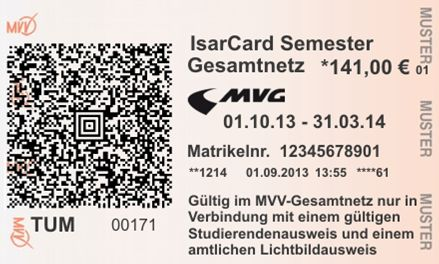
\includegraphics[width=\textwidth]{IsarCardSemester-MVG-ICA-Automat}
		%\caption{Isarcard Semester aus einem MVG-Automat}
		\label{fig:isarcardsemestermvg}
	\end{minipage}
	\quad
	\begin{minipage}[b]{0.45\linewidth}
		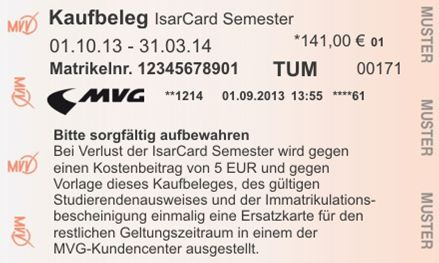
\includegraphics[width=\textwidth]{IsarCardSemester-MVG-ICA-Automat-Kaufbeleg}
		%\caption{Dazugehöriger Zahlungsbeleg}
		\label{fig:isarcardsemesterbelegmvg}
	\end{minipage}
\end{figure}

Dank des \emph{AK Mobilität zum Semesterticket München} \ref{akmobilitaet} hat
München nach vielen Jahren nun auch endlich ein Semesterticket für seine
Studenten. Bei der Zahlung deines Studienbeitrages ist dir sicherlich
aufgefallen, dass du einen Solidarbeitrag in Höhe von 59,00~€ leisten musst.
Diesen Beitrag müssen alle Studika bezahlen - im Gegenzug darf damit das
komplette Netz des MVV befahren werden: täglich von 18--6 Uhr, an Wochenenden
und Feiertagen sogar ganztägig (daher auch ``Partyticket'' genannt).


Möchtest du dein Ticket auch außerhalb dieser Zeiten nutzen, kannst du gegen
eine Zahlung von 141,00~€ an den Automaten der MVG und der
Deutschen Bahn das Semesterticket erwerben. Im Gegensatz zum Solidarbeitrag,
musst du diesen Teil des Tickets aber nicht erwerben, wenn du nicht möchtest
bzw. das Ticket nicht brauchst.

Für die meisten Studika, die den MVV nutzen, dürfte das Semesterticket die
günstige Möglichkeit sein -- es lohnt sich schon, wenn du pro Monat mehr als
23,50~€ in Fahrkarten investieren würdest.

\begin{figure}[ht]
\centering
	\begin{minipage}[b]{0.45\linewidth}
		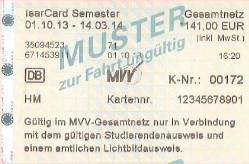
\includegraphics[width=\textwidth]{IsarCardSemester-DB-Automat}
		%\caption{Isarcard Semester aus einem DB-Automat}
		\label{fig:isarcardsemesterdb}
	\end{minipage}
	\quad
	\begin{minipage}[b]{0.45\linewidth}
		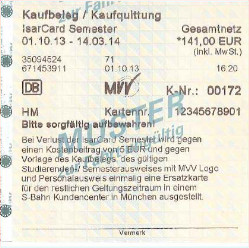
\includegraphics[width=\textwidth]{IsarCardSemester-DB-Automat-Kaufbeleg}
		%\caption{Dazugehöriger Zahlungsbeleg}
		\label{fig:isarcardsemesterbelegdb}
	\end{minipage}
\end{figure}

Das Semesterticket -- sowohl das ``Partyticket'' als auch der Teil mit
Zuzahlung -- sind immer für ein Semester gültig. Hier musst du dich auf die auf
deinem Studienausweis aufgedruckte Laufzeit des Semesters beziehen - die
anderen Hochschulen in München haben teilweise andere Laufzeiten für ihre
Semester. Bitte denke auch daran, dass das Semesterticket immer nur zusammen
mit deinem Studienausweis gilt, welcher wiederrum nur mit einem amtlichen
Ausweisdokument gültig ist.

Wenn du beschließt, ein Semesterticket am Automaten zu kaufen (halte bitte deine
Matrikelnummer zur Eingabe bereit), erhältst du zwei Belege: Ein Mal das Ticket
als solches und einen Zahlungsbeleg. Letzteren solltest du daheim gut aufheben,
denn solltest du dein Ticket verlieren, kannst du einmalig gegen Vorlage des
Zahlungsbeleges und Entrichten von 5,00~€ ein zweites Semesterticket erhalten.

\begin{urlList}
	\urlItem{http://semesterticket-muenchen.de}{akmobilitaet}
\end{urlList}

\subsection*{Ausbildungstarif}
Für Studika, die nur wenige Monate den MVV in Anspruch nehmen, kann sich unter
Umständen auch der vom MVV angebotene Ausbildungstarif II
\ref{ausbildungstarif} lohnen. Der Preis richtet sich dabei nach der Zahl der
benötigten Zeitkartenringe, die befahren werden. Bevor du dir aber ein Ticket
kaufen kannst, musst du dir eine Kundenkarte besorgen. Diese bekommst du im
MVG-Kundencenter am Hauptbahnhof, Ostbahnhof oder in der \mbox{Poccistr.}~1--3 (alle
zwischen 8:00 und 18:00~Uhr). Alternativ kannst du deine Kundenkarte auch
direkt online beantragen und selber Ausdrucken.

Das Ticket gibt es mit der Gültigkeit einer Woche (9,90~€ bis 40,40~€) oder eines Monats (36,10~€ bis 147,30~€) an einem der MVG-Zeitkartenautomaten, in den MVG-Kundencentern oder den MVG-Verkaufsstellen. Monatsfahrkarten gelten bis 12 Uhr des ersten Werktags des Folgemonats.

\begin{urlList}
	\urlItem{http://mvg-mobil.de/tarife/ausbildungstarif.html}{ausbildungstarif}
\end{urlList}

\section{Auto}
Du kommst im Allgemeinen mit dem Auto nicht schneller durch die Stadt, als mit dem ÖPNV oder dem Fahrrad. Spätestens bei der Parkplatzsuche vor der Uni wirst du dann merken, dass es bessere Möglichkeiten gibt, in die Uni zu kommen.
